\documentclass[11pt,a4paper]{article}
\usepackage[margin=21mm]{geometry}\usepackage[T1]{fontenc}\usepackage{lmodern}
\usepackage{amsmath,amssymb,booktabs,array,tikz,hyperref}
\usetikzlibrary{arrows.meta}
\setlength{\parindent}{0pt}\setlength{\parskip}{6pt}
\newcommand{\VDD}{V_{\mathrm{DD}}}
\title{2018 Homework 2\\Slew, NOR fanin and transistor scaling}
\author{NCU EE3032 Introduction to VLSI Design}\date{13 October 2026}
\begin{document}\maketitle
All four questions follow the authentic Fall 2018 PDF. The printed equations
and stated circuit models govern the derivations below. The supplied
two-page handwritten \texttt{HW2\_SOL.pdf} was read before independent
derivation. The final answers make the RC model, threshold matching and
equivalent-strength conventions explicit.

\section*{1. Why the faster rising input produces a faster falling output}
With output capacitance $C_L$, neglecting gate-drain feedthrough for the
basic explanation, charge conservation is
\[
 C_L\frac{dV_o}{dt}=I_p(V_i,V_o)-I_n(V_i,V_o).
\]
During the input's low-to-high transition, the NMOS turns on and discharges
$C_L$, while the PMOS turns off. The faster waveform $a$ reaches a larger
$V_{GS,n}$ sooner and reduces the PMOS opposing current sooner.
In long-channel saturation $I_n=\frac12\beta_n(V_i-V_{tn})^2$; consequently
the faster rise gives a larger net discharge current for the same early time
and a shorter output fall. The slow waveform $b$ spends more time with both
devices partially conducting, so discharge is weaker while the PMOS still
opposes it. Real timing also includes changing transistor regions, nonlinear
capacitance and Miller coupling, which the simple equation does not quantify.

\begin{center}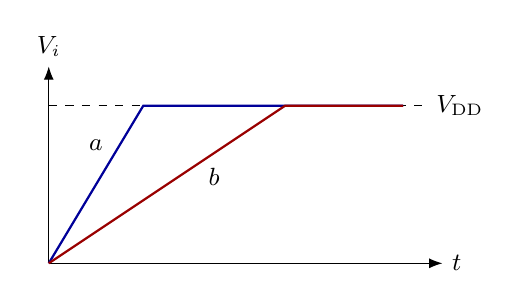
\begin{tikzpicture}[>=Latex,font=\small]
\draw[->] (0,0)--(5,0) node[right]{$t$};\draw[->] (0,0)--(0,2.5) node[above]{$V_i$};
\draw[dashed] (0,2)--(4.8,2) node[right]{$\VDD$};
\draw[blue!60!black,thick] (0,0)--(1.2,2)--(4.5,2);
\draw[red!60!black,thick] (0,0)--(3,2)--(4.5,2);
\node at (.6,1.5) {$a$};\node at (2.1,1.1) {$b$};
\end{tikzpicture}\end{center}
The supplied answer correctly emphasizes the NMOS overdrive increase.
The present derivation also accounts for the competing PMOS current and
distinguishes output fall time from input-to-output 50\% delay.
The supplementary CIC018 simulation uses explicitly illustrative sizes,
$W_p=1\,\mu$m, $W_n=0.5\,\mu$m, $L=0.18\,\mu$m, $C_L=10$ fF,
TT, 1.8 V, $25^\circ$C, and input rises of 100 ps and 1 ns.
These numerical values are not specified in the question.

\section*{2. Unloaded $n$-input NOR using a fixed-size $\pi$ model}
``Without loading'' removes external load, not the MOS diffusion
capacitances. First state a consistent fixed-size model: each NMOS has
on-resistance $R_n$, each PMOS $R_p$, and each source/drain terminal has
diffusion capacitance $C_d$. The prompt's single $R$ can be obtained by
setting $R_n=R_p=R$. Device sizes are held fixed as $n$ changes.
The NOR has $n$ series PMOS devices and $n$ parallel NMOS devices.
The output therefore has
\[
 C_o=(n+1)C_d,
\]
from one PMOS terminal and $n$ NMOS terminals. Each of the $n-1$ internal
PMOS stack nodes has $2C_d$. The source diffusion tied to the ideal supply
does not contribute to output delay.

For a rising output, all PMOS devices are on and the NMOS paths are off.
For the RC step model, initially take all stack/output capacitors discharged.
Let the internal nodes be numbered from the supply, $i=1,\ldots,n-1$.
The Elmore first moment at the output is
\begin{align*}
 \tau_r&=\sum_{i=1}^{n-1}(iR_p)(2C_d)+(nR_p)(n+1)C_d\\
 &=R_pC_d[n(n-1)+n(n+1)]
 =\boxed{2n^2R_pC_d}.
\end{align*}
The supply-to-output charging path gets longer and more internal capacitance
must be charged. Thus, for fixed sizes, $t_r$ grows quadratically with fanin.

For a falling output with exactly one NMOS on and the PMOS adjacent to the
output off, the internal chain is isolated from the output. Its exact
one-pole discharge constant and 90--10\% fall time are
\[
 \boxed{\tau_f=(n+1)R_nC_d},\qquad
 \boxed{t_f=\ln9\,(n+1)R_nC_d}.
\]
This grows linearly with fanin. If all $n$ NMOS devices switch on together,
the parallel pull-down resistance is $R_n/n$ and that same isolated-chain
case instead has $\tau_f=(n+1)R_nC_d/n$.

The falling waveform is input-pattern dependent. For example, if the PMOS
nearest the supply turns off while the other PMOS devices remain on, all
internal capacitors stay attached to the output side. The first moment is
then $R_n[(n+1)+2(n-1)]C_d=(3n-1)R_nC_d$, still linear in $n$; it is not
identical to the isolated-chain coefficient. Internal-node initial voltages
also depend on earlier input history. A unique exact fall waveform cannot
be inferred from fanin alone without specifying the switching pattern.

\textbf{Rise-time convention.} A distributed RC ladder is not a single
exponential. $\tau_r$ above is its first moment, not an exact 10--90\% rise
time. A single-pole approximation uses $t_r\simeq\ln9\,\tau_r$, while the
actual 10--90\% crossing time is measured separately. Both have the stated
fixed-size quadratic trend. The companion program records both measures.

The handwritten reference gets the qualitative quadratic/linear trends,
but uses width-scaled resistances/capacitances inconsistently when writing
its coefficient. The result above uses one explicitly defined $\pi$ model
throughout. If transistor widths are resized with fanin, both resistance
and diffusion capacitance must be changed together; the same coefficient
cannot simply be retained.

\section*{3. Mobility ratio at the inverter switching point}
At $V_i=V_o=\VDD/2$, both conducting devices are saturated for positive
thresholds below $\VDD/2$. In the ideal long-channel model with equal oxide
capacitance per area,
\[
 \tfrac12\mu_n C_{ox}(W_n/L_n)(\VDD/2-V_{tn})^2
 =\tfrac12\mu_p C_{ox}(W_p/L_p)(\VDD/2-|V_{tp}|)^2.
\]
With the given aspect ratios $(W_p/L_p)=4$ and $(W_n/L_n)=2$,
\[
 \boxed{\frac{\mu_n}{\mu_p}
 =2\left(\frac{\VDD/2-|V_{tp}|}{\VDD/2-V_{tn}}\right)^2.}
\]
Under the usual implicit matched-threshold assumption
$V_{tn}=|V_{tp}|$, this reduces to the intended answer
$\boxed{\mu_n/\mu_p=2}$, agreeing with the supplied handwritten solution.
The equality of two voltages alone does not determine mobility uniquely
when threshold magnitudes, oxide capacitances or short-channel effects are
unknown. This qualification preserves the intended course model rather
than treating the ratio as a universal BSIM3 identity.

\section*{4. Gate capacitance seen at node $x$}
The printed node $x$ drives one inverter input and one input of a two-input
NOR. The NAND's drain capacitance is explicitly excluded, as are wire
parasitics. Assume common channel length and oxide capacitance, so gate
capacitance is proportional to width.

Let inverter $W_n=w$. Since $\mu_n=2\mu_p$ and $\beta_n=\beta_p$,
the inverter has $W_p=2w$ and
$C_g=C_{ox}L(w+2w)=3C_{ox}Lw$.
To keep the two-series-PMOS NOR pull-up strength equal to the inverter's
PMOS strength, each NOR PMOS must have twice the inverter PMOS width:
$W_{p,\rm NOR}=4w$. Under the conventional worst-case \emph{one-NMOS-on}
pull-down strength definition, each NOR NMOS has $W_{n,\rm NOR}=w$.
Thus the gate capacitance of one NOR input is
\[
 C_{\rm in,NOR}=C_{ox}L(4w+w)=\frac53C_g,
 \qquad \boxed{C_x=C_g+C_{\rm in,NOR}=\frac83C_g.}
\]
\begin{center}\begin{tabular}{lrr}
\toprule Element at $x$&Normalized gate width&Capacitance\\\midrule
Inverter input&$2w+w=3w$&$C_g$\\
One NOR input&$4w+w=5w$&$5C_g/3$\\
Total&$8w$&$8C_g/3$\\\bottomrule
\end{tabular}\end{center}
This agrees with the reference answer. If $\beta_{n,eq}$ were instead
defined with \emph{both} parallel NOR NMOS devices on, each would have
half the inverter NMOS width, giving $C_x=5C_g/2$. The conventional gate
sizing answer uses the worst single conducting path; the chosen convention
is stated because the phrase ``equivalent network'' does not name a pattern.

\section*{Programs, measured evidence and source decisions}
\texttt{reproduce.py --analytical-only} checks the RC first-moment formula
for fanins 1--8, current balance with matched and unequal thresholds, and
the $8/3$ gate-capacitance ratio. These are algebraic checks.
The full command launches two actual HSPICE decks. \texttt{q1\_slew.sp}
uses the distinct CIC018 example in Q1. \texttt{q2\_pi\_rc.sp} implements
the exact stated fixed-size ideal RC model, with $R_n=R_p=1$ k$\Omega$,
$C_d=1$ fF, no external load, and a 50 fs maximum step.
It measures the normalized step-error integral, which equals the RC
first moment, separately from its 10--90\% crossing times.
Every measured first moment is checked against the independent formula;
the slower-input output fall must exceed the faster-input fall.

The two-page supplied 2018 HW2 solution is the comparison source for all
four answers. Its useful discharge-current explanation, mobility ratio
under matched assumptions, and node-capacitance result are retained.
The RC coefficient, switching-pattern dependence and missing threshold
assumptions are made explicit. Prior student numerical claims are not
presented as new process measurements. The model remains local.

Run \texttt{python reproduce.py --work PATH}; \texttt{--model PATH} and
\texttt{--hspice PATH} override the installed defaults.
The saved CSV tables and \texttt{validation.json} are included with the
report. Raw simulator files stay in the local working directory.
\section*{Recorded execution}
Both decks completed with PrimeSim HSPICE S-2021.09. The selected CIC018
inverter output fall times were $71.479047$ ps for the 100 ps input rise and
$230.642009$ ps for the 1 ns input rise, confirming the stated ordering for this
explicitly illustrative circuit. All eight ideal RC first-moment checks
agree with the formulas within 0.2\%. Selected measured RC values are:
\begin{center}\begin{tabular}{rrrrr}
\toprule $n$&$\tau_r$ (ps)&$t_r$10--90 (ps)&$\tau_f$ (ps)&$t_f$90--10 (ps)\\\midrule
1&2.000077&4.394272&2.000077&4.394272\\
2&8.000000&15.918281&3.000052&6.591564\\
4&32.000000&61.689605&5.000031&10.985996\\
8&128.000000&244.739332&9.000017&19.774959\\
\bottomrule\end{tabular}\end{center}
The table deliberately separates first moments from crossing times.
The unequal-threshold examples are algebraic current-balance tests,
not assertions about the CIC018 model's mobilities or threshold symmetry.
Every published measurement belongs to the actual run for this year.

\end{document}
